\documentclass[aspectratio=169]{beamer}
% \documentclass[handout]{beamer}
% \usepackage{pgfpages}
% \pgfpagesuselayout{2 on 1}[a4paper,border shrink=5mm]

\usepackage[utf8]{inputenc}
% \usepackage[portuguese]{babel}
\usepackage{graphicx}
\usepackage{tikz}
\usepackage{hyperref}
\usepackage{lipsum}
\usepackage{multicol}

\usepackage{./libs/solarized-light}

\usetheme{Luebeck}

\title{Data migration to Plone 5.2 and Volto}
\author{Rodrigo Ferreira de Souza}
\date{October, 2019}

% \setbeameroption{show notes on second screen=bottom}
% \setbeamertemplate{note page}[plain]

\usebackgroundtemplate{%
  \tikz\node[opacity=0.2] {
    \vbox to \paperheight{
      \vspace{14mm}
      \vfil
      \hbox to \paperwidth{
        \hfil
        
\includegraphics[height=.6\paperheight]{./img/background.png}
        \hfil
      }
      \vfil
    }
  };
}

\hypersetup{
  colorlinks=true,
  linkcolor=cyan,
  filecolor=magenta,      
  urlcolor=blue,
}

\begin{document}

\maketitle

\AtBeginSection[] {
  \begin{frame}
    \frametitle{Where we are}
    % \begin{multicols}{2}
    \setcounter{tocdepth}{1}
    \tableofcontents[currentsection]
    % \end{multicols}
  \end{frame}
}

\section{Knoledgements}
\subsection{Options to Migrate}
\begin{frame}
  \frametitle{Options to Migrate}

  \begin{columns}
    \column{.5\textwidth}
    \begin{itemize}
      \item Plone 4.3 $\rightarrow$ Plone 5+
      \begin{itemize}
        \item \href{https://github.com/collective/collective.transmogrifier}{Collective Transmogrifier} \pause
      \end{itemize}
      \item Plone 5.1 $\rightarrow$ Plone 5.2+
      \begin{itemize}
        \item \href{https://docs.plone.org/manage/upgrading/version_specific_migration/upgrade_zodb_to_python3.html}{Migrate a ZODB from Python 2.7 to Python 3} \pause
        \item \href{https://github.com/collective/collective.transmogrifier}{Collective Transmogrifier} \pause
      \end{itemize}
    \end{itemize}
    \column{.5\textwidth}
    \begin{figure}
      
\includegraphics[height=.5\textheight]{./img/002_-_transmogrifier.png}
      \caption{A transmogrifier is fictional device used for transforming one object into another object.}
    \end{figure}
  \end{columns}

  \note{
    \begin{itemize}
      \item From Plone 4.3 we just have the option to use transmogrifier
      \item For Plone 5.1 you might consider use database upgrade
      \item what means update pickle structure of ZODB to Python3 data type structure
      \item to do it you need to: run the script in Python 2; don't start the instance (important); update buildout; run tests; start instance
      \item during the process you might have problems with dependencies to fix
      \item The term was coined by Bill Waterson of Calvin and Hobbes fame
    \end{itemize}
  }
\end{frame}

\subsection{Why we use Transmogrifier?}
\begin{frame}
  \frametitle{Why we use Transmogrifier?}

  \begin{columns}
    \column{.5\textwidth}
    \begin{itemize}
      \item Have many generic Pipelines available for common cases \pause
      \item Flexibility to deal with different use cases \pause
      \item Briliant way to use Iterator Design Pattern! \pause
    \end{itemize}

    \column{.5\textwidth}
    \begin{figure}
      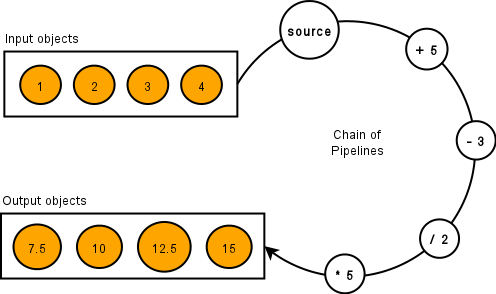
\includegraphics[width=\textwidth]{./img/001_-_Transmogrify_Diagram.png}
      \caption{Transmogrify Diagram}
    \end{figure}
  \end{columns}
  \note{
    How transmogrifier works:
    \begin{itemize}
      \item each pipeline takes the preview data items
      \item modify;
      \item and yield data to next pipeline.
    \end{itemize}
  }
\end{frame}

\begin{frame}
  \frametitle{Why we use Transmogrifier?}

  \begin{columns}
    \column{.5\textwidth}
    \begin{itemize}
      \item Have many generic Pipelines available for common cases
      \item Flexibility to deal with different use cases
      \item Briliant way to use Iterator Design Pattern!
    \end{itemize}

    \column{.5\textwidth}
    \begin{figure}
      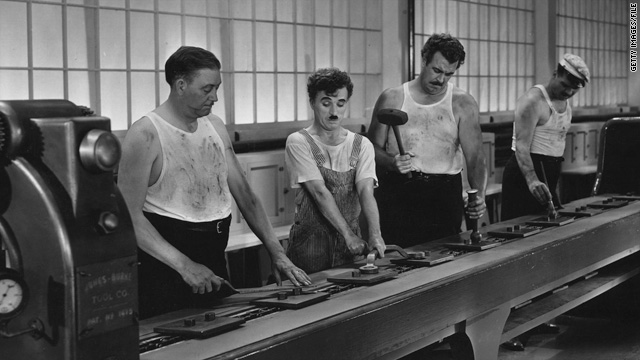
\includegraphics[width=\textwidth]{./img/001_-_modern_times.jpg}
      \caption{Modern Times -- Production line}
    \end{figure}
  \end{columns}
  \note{
    \begin{itemize}
      \item In other words, Transmogrifier allow us to create something like a production line
      \item we have an object that is modified in each pipeline
      \item until it get ready in the end.
    \end{itemize}
  }
\end{frame}

\section{Use cases}
\subsection{Large University}
\begin{frame}
  \frametitle{Large University}
  \begin{figure}
    
\includegraphics[height=.7\textheight]{./img/003_-_large_university.png}
    \caption{Large University client website}
  \end{figure}
  \note{
    \begin{itemize}
      \item Not so big database;
      \item many custom packages;
      \item a frankenstein buildout.
    \end{itemize}
  }
\end{frame}

\subsection{High-profile government client}
\begin{frame}
  \frametitle{High-profile government client}
  \begin{figure}
    
\includegraphics[height=.7\textheight]{./img/004_-_government_client.jpg}
    \caption{High-profile government client website}
  \end{figure}
  \note{
    \begin{itemize}
      \item Many data;
      \item Migration takes around 4 hours to run;
      \item some addons;
      \item custom report object type;
      \item was 1 archetypes, becomes 10 dexterity.
    \end{itemize}
  }
\end{frame}

\subsection{One of the largest research institutions in Germany}
\begin{frame}
  \frametitle{One of the largest research institutions in Germany}
  \begin{figure}
    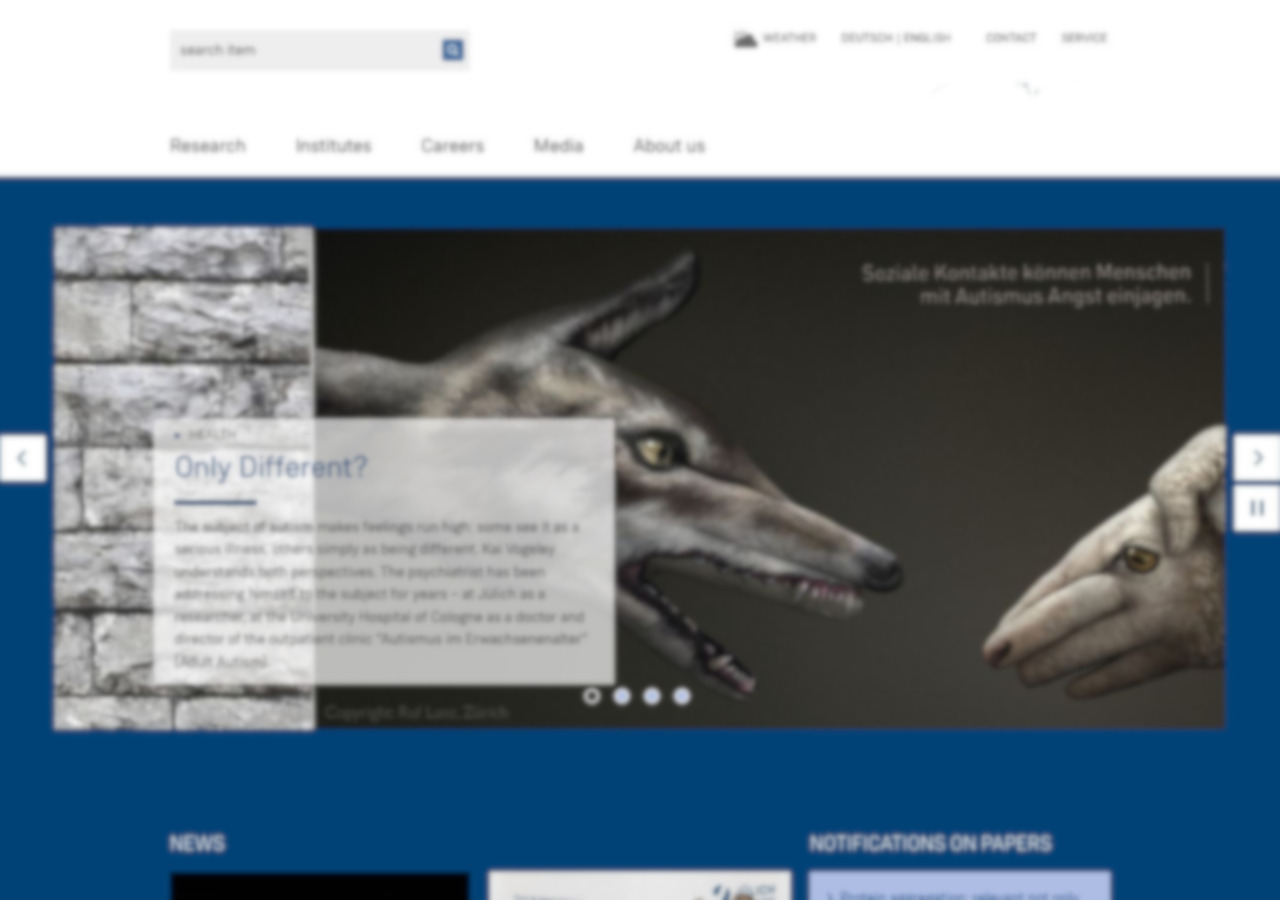
\includegraphics[height=.7\textheight]{./img/005_-_research_institution.jpg}
    \caption{Large research institution client website}
  \end{figure}
  \note{
    \begin{itemize}
      \item Intranet;
      \item Had a third part system integration that needs to be imported in new website.
    \end{itemize}
  }
\end{frame}

\section{The challendge}
\subsection{The challendge}
\begin{frame}
  \frametitle{The challendge}
  \begin{itemize}
    \item From:
    \begin{itemize}
      \item Python 2.x \pause
      \item Plone 4.3.x or 5.0.x or 5.1.x \pause
      \item Archetypes or Dexterity \pause
      \item Old Products \pause
      \item Sometimes other systems \pause
    \end{itemize}
    \item To:
    \begin{itemize}
      \item Python 3 \pause
      \item Plone 5.2 \pause
      \item Volto
    \end{itemize}
  \end{itemize}
  \note{
    So.. to sum up, those are the things that we need to do
  }
\end{frame}

\subsection{Advantages for the clients}
\begin{frame}
  \frametitle{Advantages for the clients}
  \begin{itemize}
    \item They spare a migration from Plone 5 to Plone 6 \pause
    \item At least part of it
  \end{itemize}
  \note{
    For the clients they can spare part of the Plone 5 to Plone 6 migration
  }
\end{frame}

\subsection{Advantages for Plone solutions providers}
\begin{frame}
  \frametitle{Advantages for Plone solutions providers}
  \begin{itemize}
    \item A way to sell clients the Python 3 upgrade \pause
    \item Which is costly but does not gain the client anything in terms of functionality
  \end{itemize}
  \note{
    For the soluctions providers we can sell together Python 3 with Volto
  }
\end{frame}

\section{Our way}
\subsection{Packages}
\begin{frame}
  \frametitle{Packages}
  \begin{itemize}
    \item \href{https://github.com/kitconcept/kitconcept.contentcreator}{kitconcept Content Creator} \pause
    \item \href{https://github.com/kitconcept/migration-plone5/tree/master/src/kitconcept.migrator}{kitconcept Migrator} \pause
    \item \href{https://github.com/kitconcept/migration-plone5}{Migration Plone 5}
  \end{itemize}
  \note{
    k.migrator lives inside the Migration Package
  }
\end{frame}

\subsection{Commander Utility}
\begin{frame}
  \frametitle{Commander Utility}
  \begin{figure}
    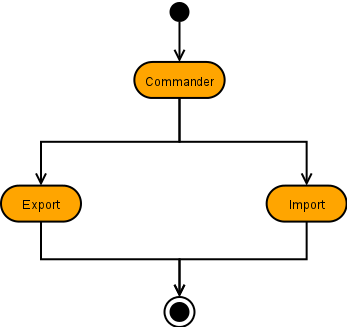
\includegraphics[height=.7\textheight]{./img/006_-_Commander_Utility.png}
    \caption{Commander Utility}
  \end{figure}
  \note{
    We created an utility to help orchestrate the migration process.
  }
\end{frame}

\subsection{Jenkins}
\begin{frame}
  \frametitle{Jenkins}
  \begin{figure}
    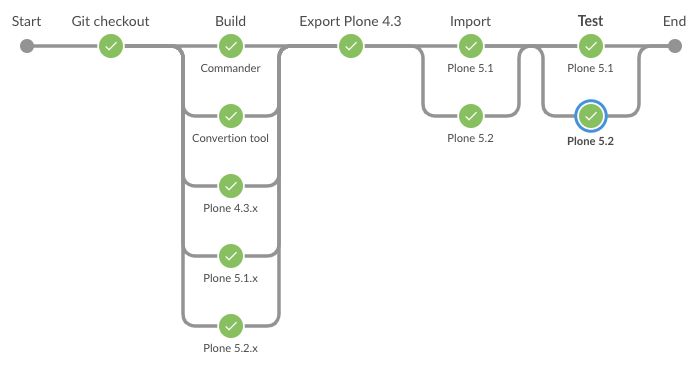
\includegraphics[height=.7\textheight]{./img/007_-_Jenkins.png}
    \caption{Jenkins}
  \end{figure}
  \note{
    Each commit runs all those steps to make tests (smoke tests).
  }
\end{frame}

\subsection{Migration Server}
\begin{frame}
  \frametitle{Migration Server}
  \begin{figure}
    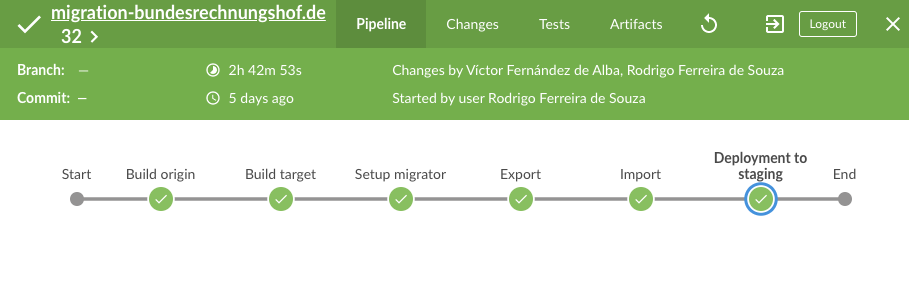
\includegraphics[width=\textwidth]{./img/008_-_Migration.png}
    \caption{Migration Server}
  \end{figure}
  \note{
    Also we have migration Jenkins node, that we push the button to start the migration (what takes about 4 hours to finish)
  }
\end{frame}

% \section{Live codding}
% \subsection{Our general approach}
% \begin{frame}
%   \frametitle{Our general approach}
%   \begin{figure}
%     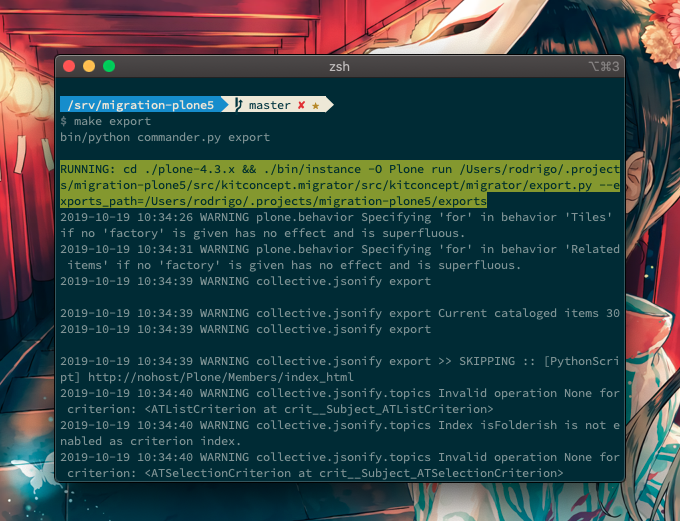
\includegraphics[height=.7\textheight]{./img/009_-_our_way.png}
%     \caption{Running migrator by hand}
%   \end{figure}
% \end{frame}

\section{Details on how we did things}
\subsection{General Backend}
\begin{frame}
  \frametitle{General Backend}
  \begin{itemize}
    \item ATTopics $\rightarrow$ Collection \pause
    \item RichText $\rightarrow$ Volto Blocks \pause
    \item Portlets \pause
    \item Postmigration
  \end{itemize}
  \note{
    \begin{itemize}
      \item For ATTopics our strategy was to fix during export phase
      \begin{itemize}
        \item we basically run the default Plone upgrade step on the query,
        \item and make the changes while still at Plone 4.3
        \item and make the exported data ready for dexterity collections
      \end{itemize}
      \item For tinymce html to volto,
      \begin{itemize}
        \item we created a simple nodejs code that convert to DraftJS data,
        \item so for each object we call this utility with our HTML,
        \item and set the result in tile behaviour attribute.
      \end{itemize}
      \item Portlets are migrated, but not showed in Volto;
      \begin{itemize}
        \item we have one case with a special portlet that have a download URL that points to other part of the website;
        \item so we need to keep track of this data.
      \end{itemize}
      \item Postmigration are some "not migrated" data (c.cover for example)
      \begin{itemize}
        \item that we should replace for something else after migration,
        \item so we automated it creating some data manually
        \item and saving the JSON extracted by restapi from this content.
      \end{itemize}
    \end{itemize}
  }
\end{frame}

\subsection{The Volto part}
\begin{frame}
  \frametitle{The Volto part}
  \begin{itemize}
    \item What we Polish to enter in Volto land:
    \begin{itemize}
      \item \href{https://github.com/collective/collective.folderishtypes}{Use Collective Folderish Types} \pause
      \item Deal with default pages \pause
      \item Convert RichText HTML to Volto DraftJS (node utility) \pause
      \item Easily point to old website when content not imported \pause
      \item Fix URLs (planned resolveuid) \pause
      \item Simple Folders $\rightarrow$ Document with Collection Block (planned) \pause
      \item Simple Collection $\rightarrow$ Document with Collection Block (planned)
    \end{itemize}
  \end{itemize}
  \note{
    \begin{itemize}
      \item We use c.folderishtypes because in volto we don't have the concept of default pages, so for migration we need to make almost everything folderish to keep in sync the old and new website URLs
      \item Some content types of old website is NOT going to be imported, in this case we write some code to show a link to point to the old website
      \item Well we still don't have resolveuid concept in volto.. we plan to use something similar to what Plone does for tinymce, but with restapi and volto
      \item Folders will be as simple document with listing block showing the folder content
      \item Collections becomes simple cocument with listing block running the collection query
    \end{itemize}
  }
\end{frame}

\begin{frame}
  \frametitle{Questions?}
  \begin{figure}
    
\includegraphics[height=.7\textheight]{./img/010_-_questions.jpg}
  \end{figure}
\end{frame}

\begin{frame}
  \begin{figure}
    
\includegraphics[height=.7\textheight]{./img/011_-_thanks.jpg}
  \end{figure}
\end{frame}

% \section{Code example}
% \subsection{Code example}
% \begin{frame}[fragile]
%     \frametitle{Code example}
%     \begin{lstlisting}[language=python]
% @implementer(IBlocksTransformEnabled)
% class View(BrowserView):

%     """Default view, a compose page."""

%     index = ViewPageTemplateFile(
%         'templates/view.pt')

%     def __call__(self):
%         # forbid image indexing as scales are volatile
%         self.request.RESPONSE.setHeader(
%             'X-Robots-Tag', 'noimageindex')
%         return self.index()
%     \end{lstlisting}
% \end{frame}

\end{document}
